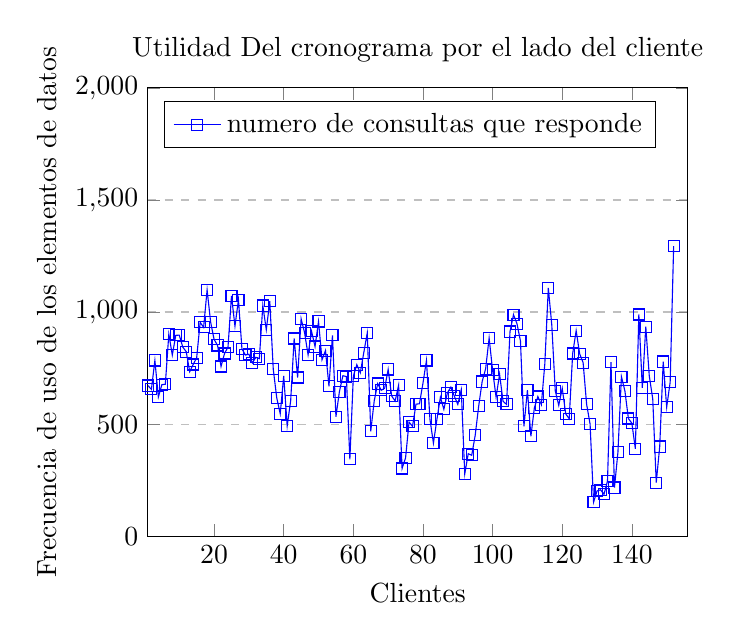
\begin{tikzpicture}
\begin{axis}[
    title={Utilidad Del cronograma por el lado del cliente},
    xlabel={Clientes},
    ylabel={Frecuencia de uso de los elementos de datos},
    xmin=1, xmax=156,
    ymin=0, ymax=2000,
    xtick={},
    ytick={},
    legend pos=north west,
    ymajorgrids=true,
    grid style=dashed,
]

\addplot[
    color=blue,
    mark=square,
    ]
    coordinates {
    %USO EXACTO
   (1,672)
(2,655)
(3,784)
(4,621)
(5,676)
(6,678)
(7,901)
(8,808)
(9,896)
(10,897)
(11,844)
(12,823)
(13,734)
(14,766)
(15,796)
(16,954)
(17,932)
(18,1099)
(19,956)
(20,878)
(21,851)
(22,757)
(23,815)
(24,844)
(25,1072)
(26,937)
(27,1055)
(28,836)
(29,808)
(30,812)
(31,773)
(32,798)
(33,792)
(34,1029)
(35,921)
(36,1048)
(37,745)
(38,617)
(39,546)
(40,715)
(41,492)
(42,604)
(43,882)
(44,708)
(45,970)
(46,907)
(47,809)
(48,914)
(49,846)
(50,958)
(51,787)
(52,828)
(53,669)
(54,896)
(55,533)
(56,645)
(57,716)
(58,712)
(59,343)
(60,714)
(61,765)
(62,729)
(63,819)
(64,907)
(65,468)
(66,604)
(67,681)
(68,651)
(69,660)
(70,744)
(71,626)
(72,603)
(73,673)
(74,302)
(75,349)
(76,509)
(77,490)
(78,589)
(79,591)
(80,683)
(81,784)
(82,522)
(83,415)
(84,521)
(85,620)
(86,566)
(87,639)
(88,665)
(89,625)
(90,588)
(91,654)
(92,278)
(93,368)
(94,361)
(95,450)
(96,580)
(97,690)
(98,747)
(99,884)
(100,740)
(101,620)
(102,723)
(103,602)
(104,588)
(105,913)
(106,988)
(107,948)
(108,871)
(109,490)
(110,651)
(111,446)
(112,573)
(113,623)
(114,587)
(115,769)
(116,1108)
(117,942)
(118,648)
(119,584)
(120,660)
(121,546)
(122,524)
(123,815)
(124,917)
(125,814)
(126,774)
(127,589)
(128,500)
(129,152)
(130,202)
(131,207)
(132,187)
(133,246)
(134,777)
(135,217)
(136,375)
(137,712)
(138,648)
(139,525)
(140,504)
(141,390)
(142,989)
(143,662)
(144,935)
(145,715)
(146,612)
(147,239)
(148,400)
(149,779)
(150,576)
(151,687)
(152,1294)
    };
    \legend{numero de consultas que responde}

\end{axis}
\end{tikzpicture}

